\documentclass{report}
\usepackage{amsmath}
\usepackage{graphicx}
\graphicspath{ {./diagrams/} }

\begin{document}
\chapter{Introduction to Chaos in the Lorenz System}
\section{Preamble}
In higher dimensions, nonlinear systems of differential equations have the
potential to act in ways not possible in one or two-dimensional systems. In 
two-dimensional systems, for instance, any trajectory that can be contained within a closed, bounded subset of the plane will either approach a fixed point
(if it exists), or, if the fixed point is excluded from R, the trajectory is
either a closed orbit or approaches one asymptotically. In effect, this proves
that if we can 'trap' a trajectory within a bounded region, then we expect its 
long-term behavior to be periodic or fixed.
	
As we move to three dimensions this result no longer holds. A solution to a
dynamical system can be shown to stay within a closed, bounded region yet
never settle into any predictable long-term behavior. Furthermore, solutions 
that begin with similar initial conditions may actually fly apart in the 
system, so that it becomes difficult to extrapolate the motion of a trajectory 
from the starting point. These traits fall under the definition of chaos in a
dynamic system. The term \emph{chaos} in this context is distinguished from
being nondeterministic or random. We reference the definition of chaos
suggested by Strogatz\cite{strogatz15}: "Chaos is aperiodic long-term behavior
in a deterministc system that exhibits sensitive dependence on initial
conditions." A chaotic system is aperiodic in that as \(t \rightarrow \infty\),
trajectories do not approach any fixed points, periodic orbits, or quasiperiodic
orbits, deterministic in that no noise or random information is a part of the
system, and sensitive in that neighboring trajectories tend to move far apart.

The goal of our report is to explore the basics of dynamical 
chaos through an analysis of the Lorenz equations, relying on computer
simulation when deriving the behavior of the system by hand proves intractable.

\section{Fixed Point Analysis}

We first state the Lorenz equations:
\begin{align*}
   \dot{x} = \sigma y - \sigma x \\
   \dot{y} = rx - y - xz \\
   \dot{z} = xy - bz
\end{align*}
where \( \sigma , b, and r \) are parameters greater than zero. Our first goal is to
locate the fixed points of the system and identify their behavior. Setting
\( \dot{x}, \dot{y}, and \dot{z}\) to zero, we have
\begin{align*}
   x = y \\
   (r-z)x - y = 0 \\
   xy = bz
\end{align*}
Replacing y with x as given in the first equation:
\begin{align*}
  x = y \\
  (r-z-1)x = 0 \longrightarrow x = 0 or z = r-1 \\
  x^2 = bz
\end{align*}

We see that three fixed points are possible: \( \boldsymbol{x\mbox{*}} = (0,0,0),(\sqrt{b(r-1)},\sqrt{b(r-1)},r-1)\), and \((-\sqrt{b(r-1)},-\sqrt{b(r-1)},r-1)\).
The fixed point at the origin exists for all choices of r, while the symmetric 
pair of fixed points will only exist if \(r > 1\). In fact, a supercritical 
pitchfork bifurcation occurs at the origin when \( r = 1 \).

The Jacobian matrix for the Lorenz system i
\[
\begin{bmatrix}
   -\sigma & \sigma & 0 \\
   r - z & -1 & -x \\
   y & x & -b
\end{bmatrix}
\]

For the fixed point at the origin, the linearization of the system becomes
\[
\begin{bmatrix}
   -\sigma & \sigma & 0 \\
   r & -1 & 0 \\
   0 & 0 & -b

\end{bmatrix}
\]
The z component decays exponentially, while the behavior of x and y depends on 
r: for \( r < 1\), the determinant of the matrix containing only x and y is
\(\sigma - r\sigma > 0\), and the trace is negative. We find the discriminant 
\(tr^2 - 4det = \sigma^2 +2\sigma + 1 -4(\sigma -r\sigma) = (\sigma - 1)^2 +
  4r\sigma\). Since r and \(\sigma > 0 \), we have \(tr^2 -4det > 0\), which 
means that the fixed point at the origin is a stable node. When \(r > 1\), on 
the other hand, the origin changes stability and becomes a saddle node, and the
fixed points \(C^+\) and \(C^-\) appear. If this is a supercritical pitchfork
bifurcation we expect these to be stable.

The linearization of \(C^+\) and \(C^-\) is as follows:
\[
\begin{bmatrix}
   -\sigma & \sigma & 0 \\
   1 & -1 & -d \\
   d & d & -b
\end{bmatrix}
\]
Where \(d = \pm \sqrt{b(r-1)}\). When we derive the characteristic polynomial 
for this linearization we find that they are identical, so we only show the
process for positive \(d\). Now we see that the behavior of z is no longer
decoupled from x or y, so we cannot simplify the analysis to the 2-dimensional
case. Instead, we find the eigenvalues directly:
\begin{align*}
  det(A-\lambda I) = (-\sigma-\lambda)((-1-\lambda)(-b-\lambda)+d^2 )-
  \sigma(-b-\lambda+d^2) \\
  \quad = (\lambda^2 +(\sigma+1)\lambda+\sigma)(-b-\lambda)+
d^2(-\sigma-\lambda)+b\sigma+\sigma\lambda-\sigma d^2 \\
  \quad = (-1)(\lambda^3 +(\sigma + b + 1)\lambda^2 +(b\sigma+\sigma+b)\lambda
+b\sigma)+b\sigma+(\sigma-d^2)\lambda-2\sigma d^2
\end{align*}
We let \(det(A-\lambda I) = 0\), which allows us to simplify the polynomial
into its most useful form:
\begin{align*}
  det(A-\lambda I) = \lambda^3 + (\sigma+b+1)\lambda^2 + b(\sigma+r)\lambda
+ 2\sigma b(r-1) = 0
\end{align*}
Finding the eigenvalues for this linearization for certain parameter values
is computationally laborious, but possible. When we set \(\sigma = 10\),
\(b=8/3\), and vary our choice of \(r\), we find that for some r we get
complex eigenvalues with negative real part, implying that \(C^+\) and \(C^-\)
are stable spirals at some point. To show this analytically, we will actually
find the value of \(r\) at which a pair of purely imaginary solutions appear.
We call this value \(r_H\), and by deriving this we learn that \(C^+\) and
\(C^-\) undergo Hopf bifurcations. 

Suppose we do have a pair of purely imaginary eigenvalues \(\lambda = \pm
i\omega\), where \(\omega\) is real, and that \( \sigma > b+1 \). Then the
characteristic polynomial is re-expressed as a complex number (it suffices
just to use the positive imaginary eigenvalue):
\begin{align*}
   -i\omega^3 - (\sigma + b + 1)\omega^2 + ib(\sigma + r)\omega
+ 2\sigma b(r-1) = 0 \\
   \rightarrow i(-\omega^3 +\omega b(\sigma + r) + 2\sigma b(r-1)) -
(\sigma+b+1)\omega^2 = 0
\end{align*}
Since \(\omega\) and the parameters are all real, the above implies both
the real and imaginary parts of the equation must equal 0 as well. From this
we find a pair of equations:
\begin{align*}
   -\omega^3 +\omega b(\sigma+r) = 0 \\
   -(\sigma +b+1)\omega^2 + 2\sigma b(r-1) = 0
\end{align*}
Our goal is to find an expression for \(r\). Through some rearrangement we
get
\begin{align*}
   b(\sigma+r) = \omega^2 \\
   \frac{2\sigma b(r-1)}{\sigma +b+1} = \omega^2 
\end{align*}
which we can merge into one equation that we rewrite to isolate r, and so
obtain the Hopf bifurcation value:
\begin{align*}
   2\sigma br -(\sigma +b+1)br = b\sigma(\sigma+b+1)+2\sigma b \\
   \rightarrow r = r_H = \sigma \frac{\sigma+b+3}{\sigma-b-1}
\end{align*}
Note that our assumption that \( \sigma > b+1 \) was necessary, or else we
either fail to derive the equation for r, or the equation implies r is
negative, a contradiction to our constraints on the parameters. A symbolic
solver in Mathematica confirms our derivation of \(r_H\) and also tells us
that the third eigenvalue is \(\lambda = -1-b-\sigma\), which is negative.
The computation can be found in the corresponding Mathematica notebook file.

Unfortunately this does not give any information as to whether \(C^+\) and
\(C^-\) at \(r_h\) are supercritical or subcritical, but knowing that they
are Hopf bifurcations does confirm that they are locally stable spirals for
\(r < r_h\). Combined with the fact that the third eigenvalue is negative,
we conclude that before the bifurcations \(C^+\) and \(C^-\) are stable.
It has been shown that the bifurcation is in fact subcritical\cite{strogatz15}
\cite{sparrow82}, which means that soon after the bifurcation, the (unstable)
limit cycles disappear and all fixed points of the system are unstable. This
sets up the conditions under which the Lorenz sytem behaves chaotically.

\section{Properties of the Lorenz System Leading to the Strange Attractor}

When \(r\) passes the Hopf bifurcation value \(r_H\), it is unclear how
trajectories in the system will behave. Do new limit cycles appear? Do
trajectories approach infinity? We prove a couple of properties of the Lorenz
system that effectively bound the long-term behavior of its trajectories.

First we show that the Lorenz equations form a volume-dissipating system. The
derivation appears in Strogatz\cite{strogatz15}, but we reproduce it here.
We let the Lorenz system be represented by a vector function
\(\boldsymbol{f}(\boldsymbol{x})\), and \(V(t)\) a volume whose value changes
with respect to the Lorenz system, with surface \(S(t)\). Then
\begin{align*}
  \dot{V} = \int_S (\boldsymbol{f}\cdot\boldsymbol{n}dA
\end{align*}
and by the divergence theorem:
\begin{align*}
  \dot{V} = \int_V \nabla\cdot\boldsymbol{f}dV \\
  \nabla\cdot\boldsymbol{f} = \frac{\partial}{\partial x}[\sigma(y-x)]
+\frac{\partial}{\partial y}[rx-y-z] + \frac{\partial}{\partial z}[xy-bz] \\
  \rightarrow = -\sigma -1-b < 0 
\end{align*}
The divergence here is constant and negative, which means volumes \(V\) shrink
exponentially fast.

A second, analogous property is that an ellipsoid exists so that all
trajectories eventually enter it and stay in there forever. Let there be an
ellipsoid of form \(rx^2 +\sigma y^2+\sigma(z-2r)^2 \leq C\).

\section{Transition to Chaos}

Given what we have learned about the Lorenz system, we know trajectories will
not trend towards infinity, and for many values of \( r > r_H\), no new limit
cycles appear. (There are windows of r where in fact new period cycles appear,
but we will cover that later.) In that case, numerical experiments show that
trajectories begin to behave chaotically. In the analysis to follow, we use
numerical computation to generate trajectories and their component graphs, and
we select pairs of trajectories and plot the distance between them over time.
The scope of our paper is limited, so we defer use of more analytical tools.

\section{Changes over Parameter Space over \(r\)}

Using Mathematica, we generated diagrams that map out the changes in the
Lorenz system as r changes. See that for \(r < 1\) that only one fixed point
exists and all trajectories funnel towards it, but as \(r\) increases two new
fixed points are generated, and a distinct palmier shape is drawn out by
the trajectories. Note that, for our calculations, we set \(\sigma = 10\) and
\(b = 8/3 \) fixed for all values of \(r\), in accordance with Lorenz's
original experiments. This means \(r_H \approx 24.7\).

\begin{figure}[h]
  \centering
  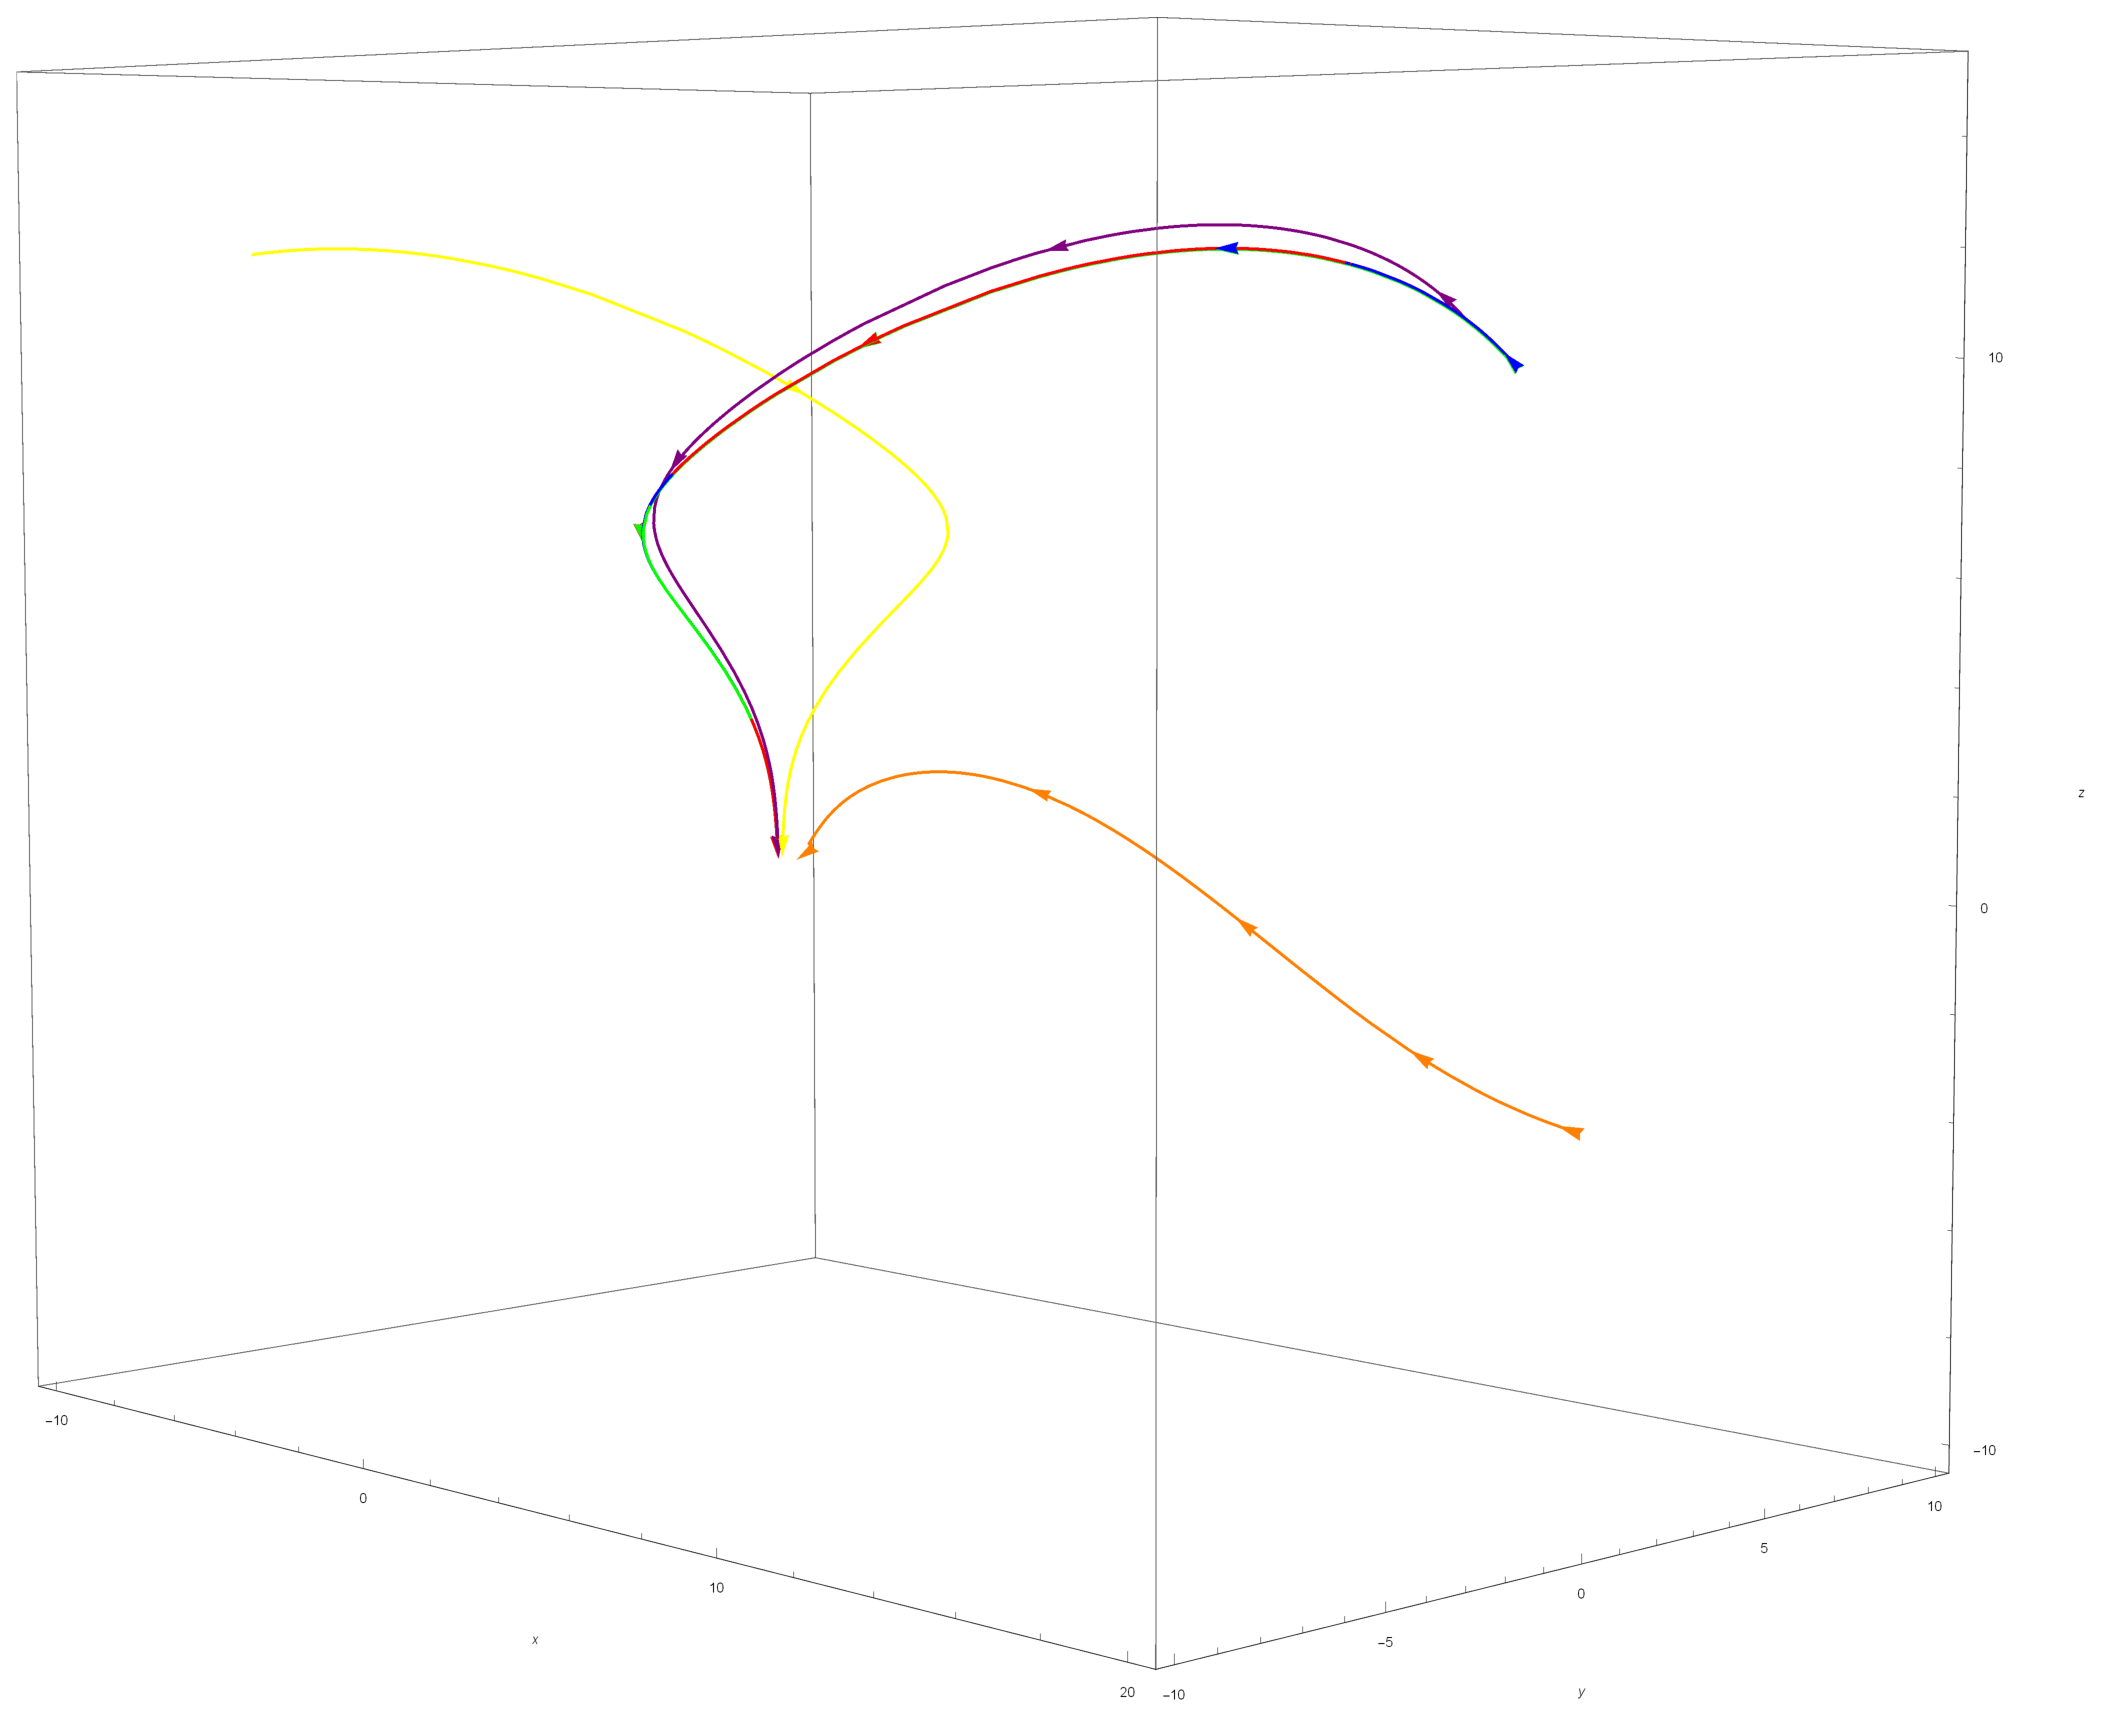
\includegraphics[width=0.75\textwidth]{r0.5.eps}
  \caption{Plot of selected trajectories for r = 0.5}
  \label{fig:r_small}
\end{figure}
Figure \ref{fig:r_small} exhibits trajectories that move in in oblique arcs
as the z component dissipates.
\begin{figure}[h]
  \centering
  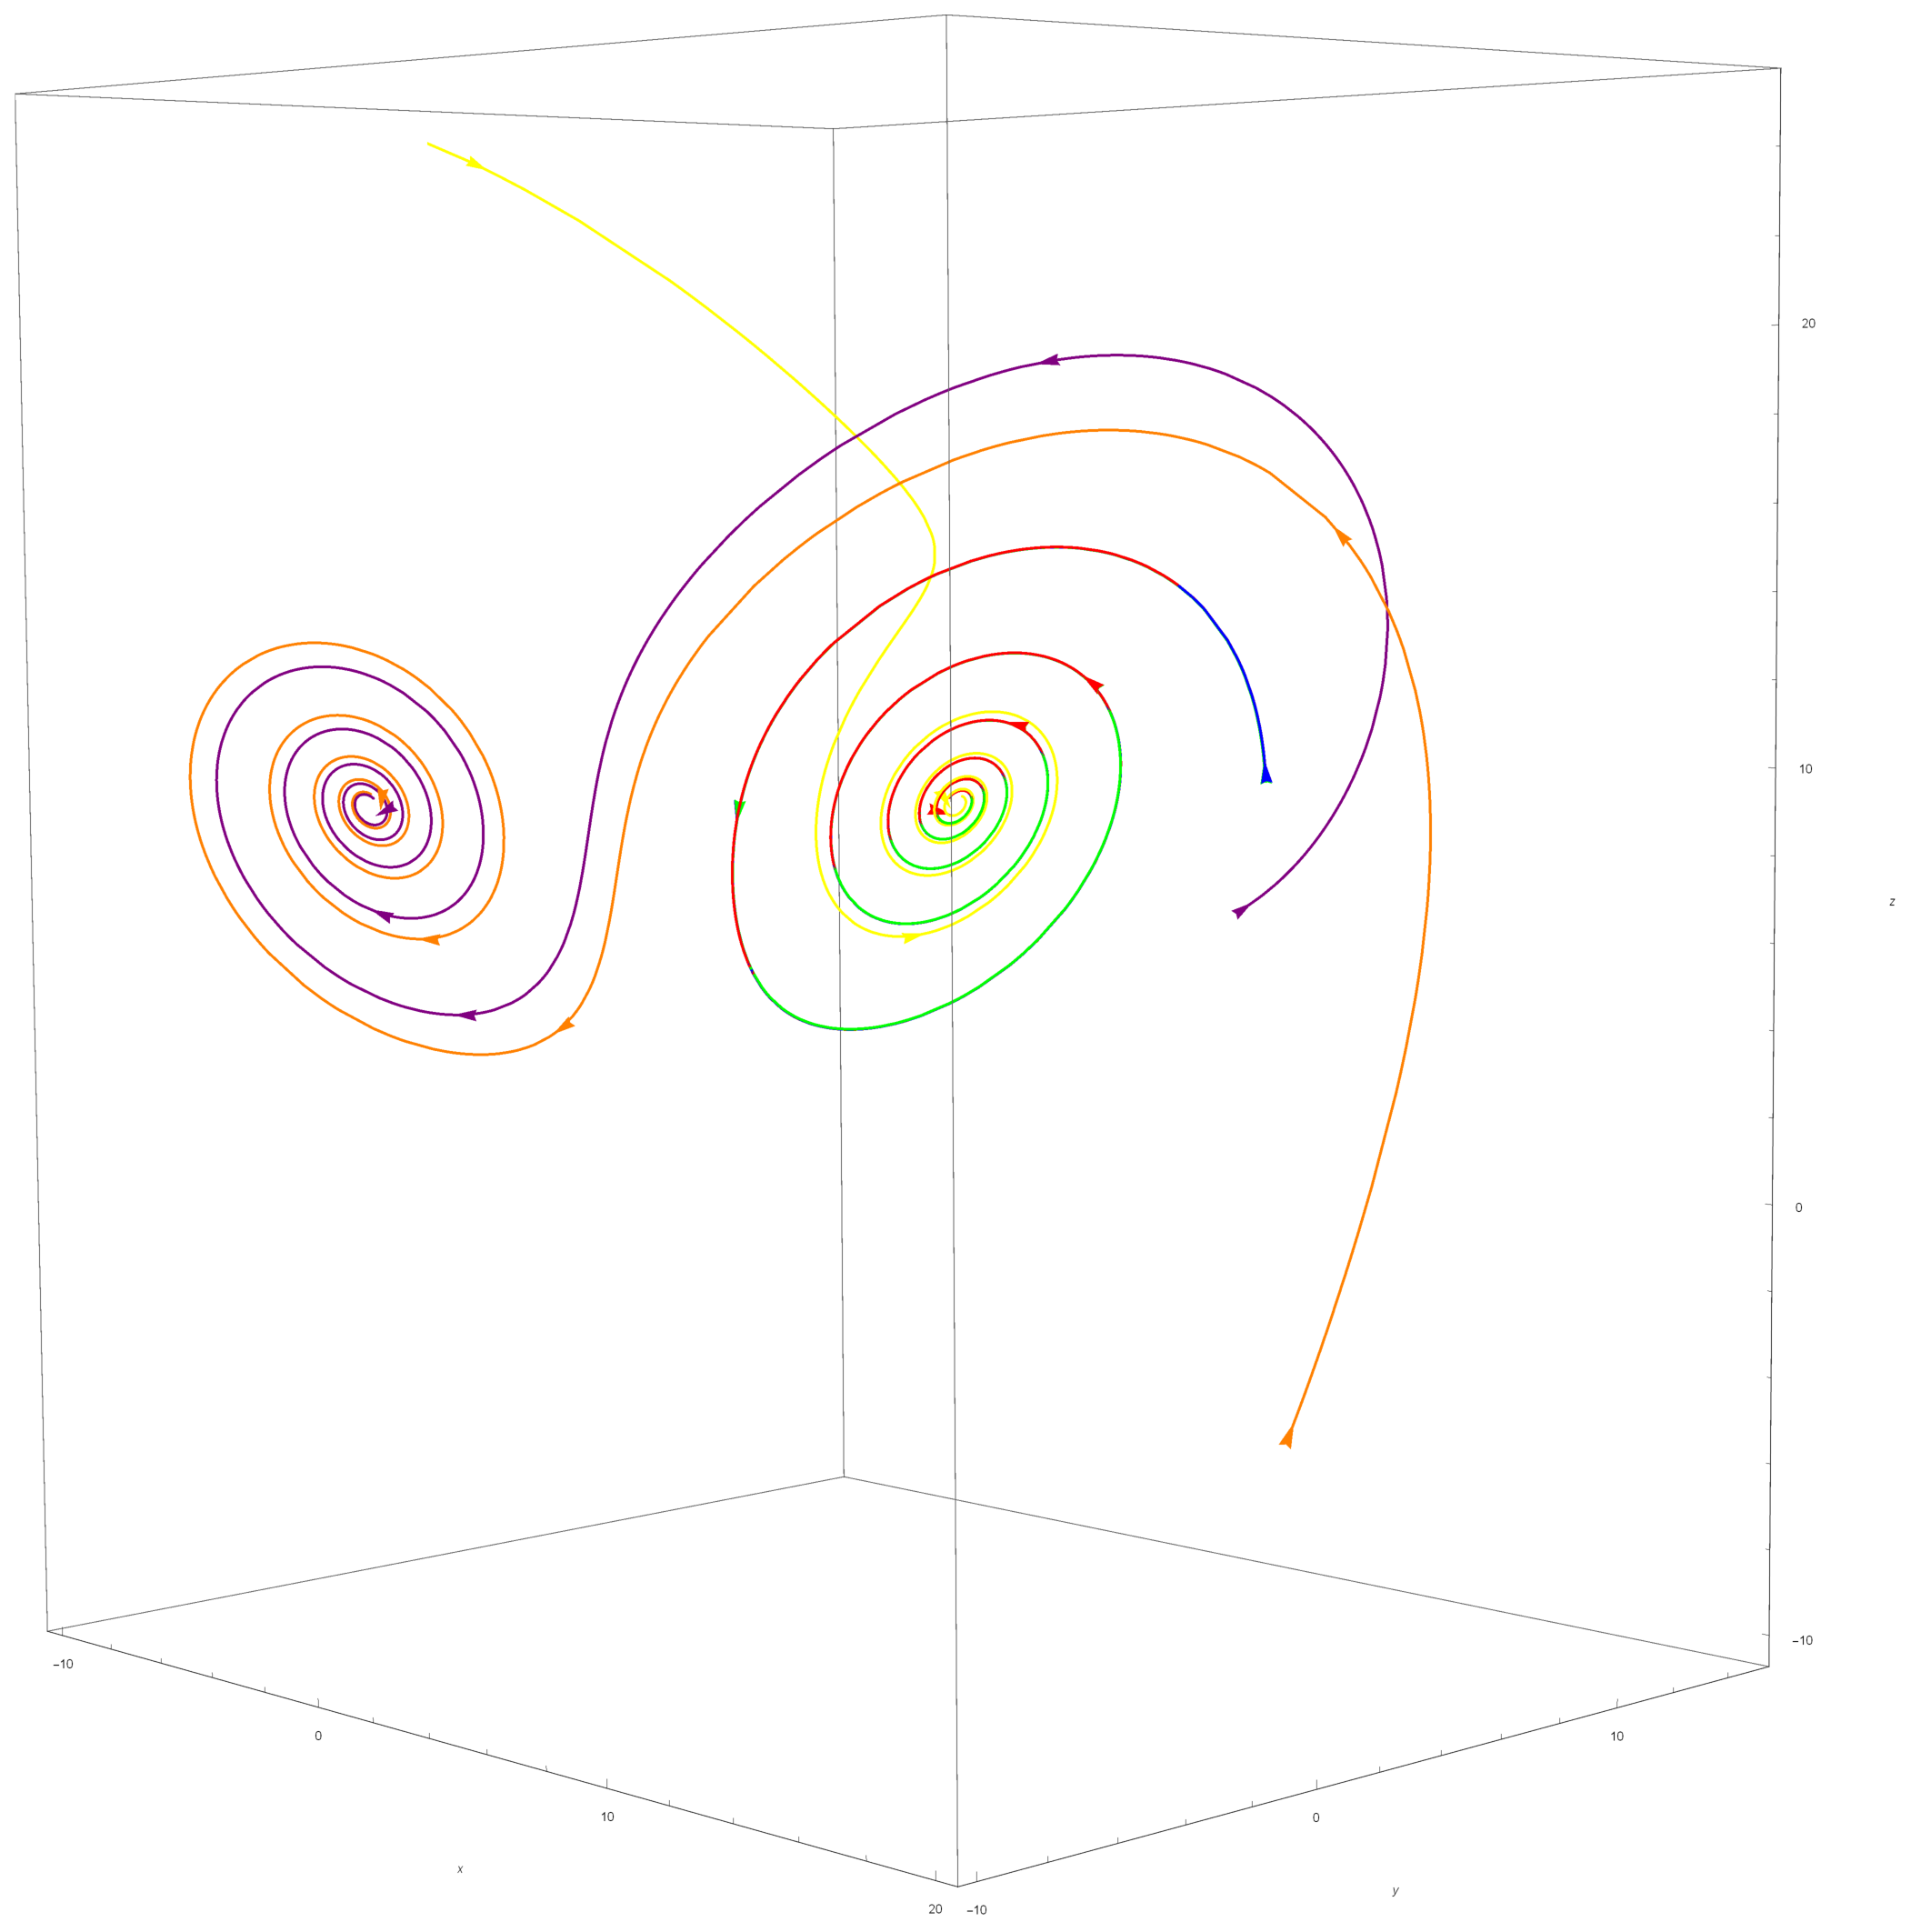
\includegraphics[width=0.75\textwidth]{r10.eps}
  \caption{Trajectories for r = 10}
  \label{fig:r_10}
\end{figure}

\begin{figure}[h]
  \centering
  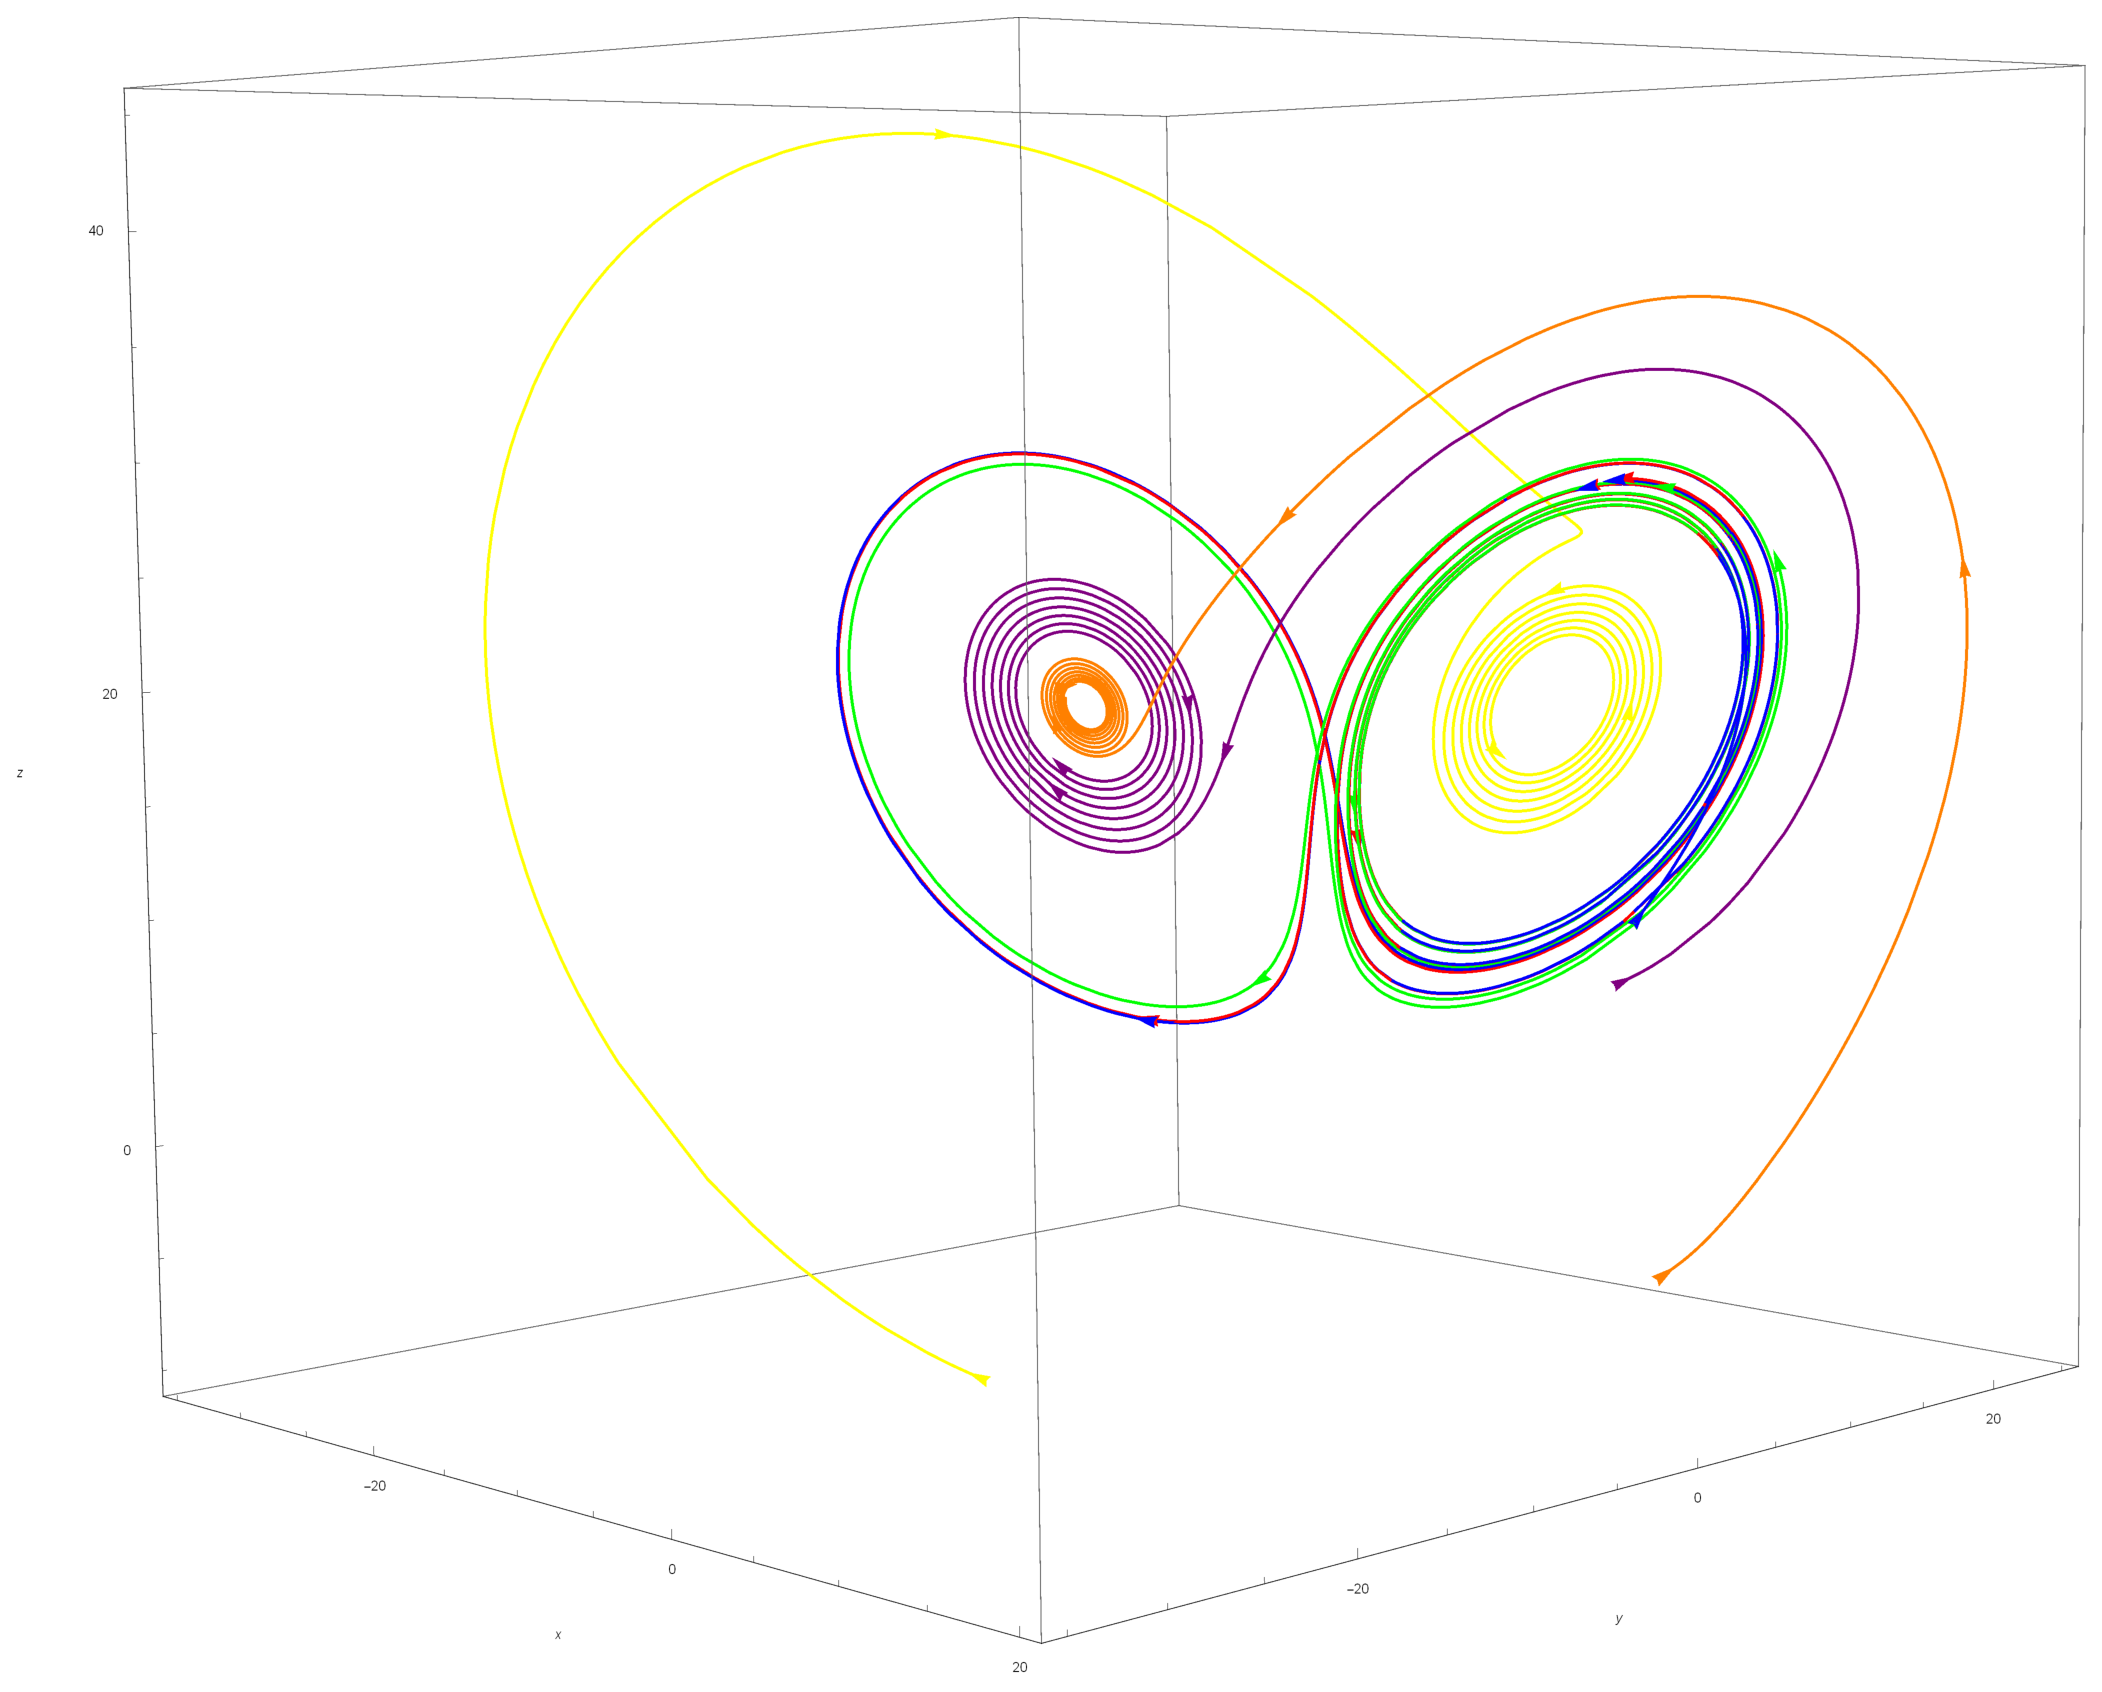
\includegraphics[width=0.75\textwidth]{r20.eps}
  \caption{Trajectories for r = 20}
  \label{fig:r_20}
\end{figure}
The next two figures illustrate what happens around the two new fixed points
\(C^+\) and \(C^-\). We see that in Figure \ref{fig:r_10} the purple and
orange trajectories begin on one side of the figure but both spiral into one
fixed point, while the red and blue trajectories begin close enough to the
other fixed point to remain there. By r = 20, some trajectories are progressing
towards their fixed points but others are volleyed in between the two lobes.
Current literature describes this phenomenon as "intermittent chaos": short
term trajectories move around aperiodically before reaching a fixed point,
and as we see, the time it may take before a trajectory is 'trapped' within
the radius of a fixed point can vary.

\begin{figure}[h]
  \centering
  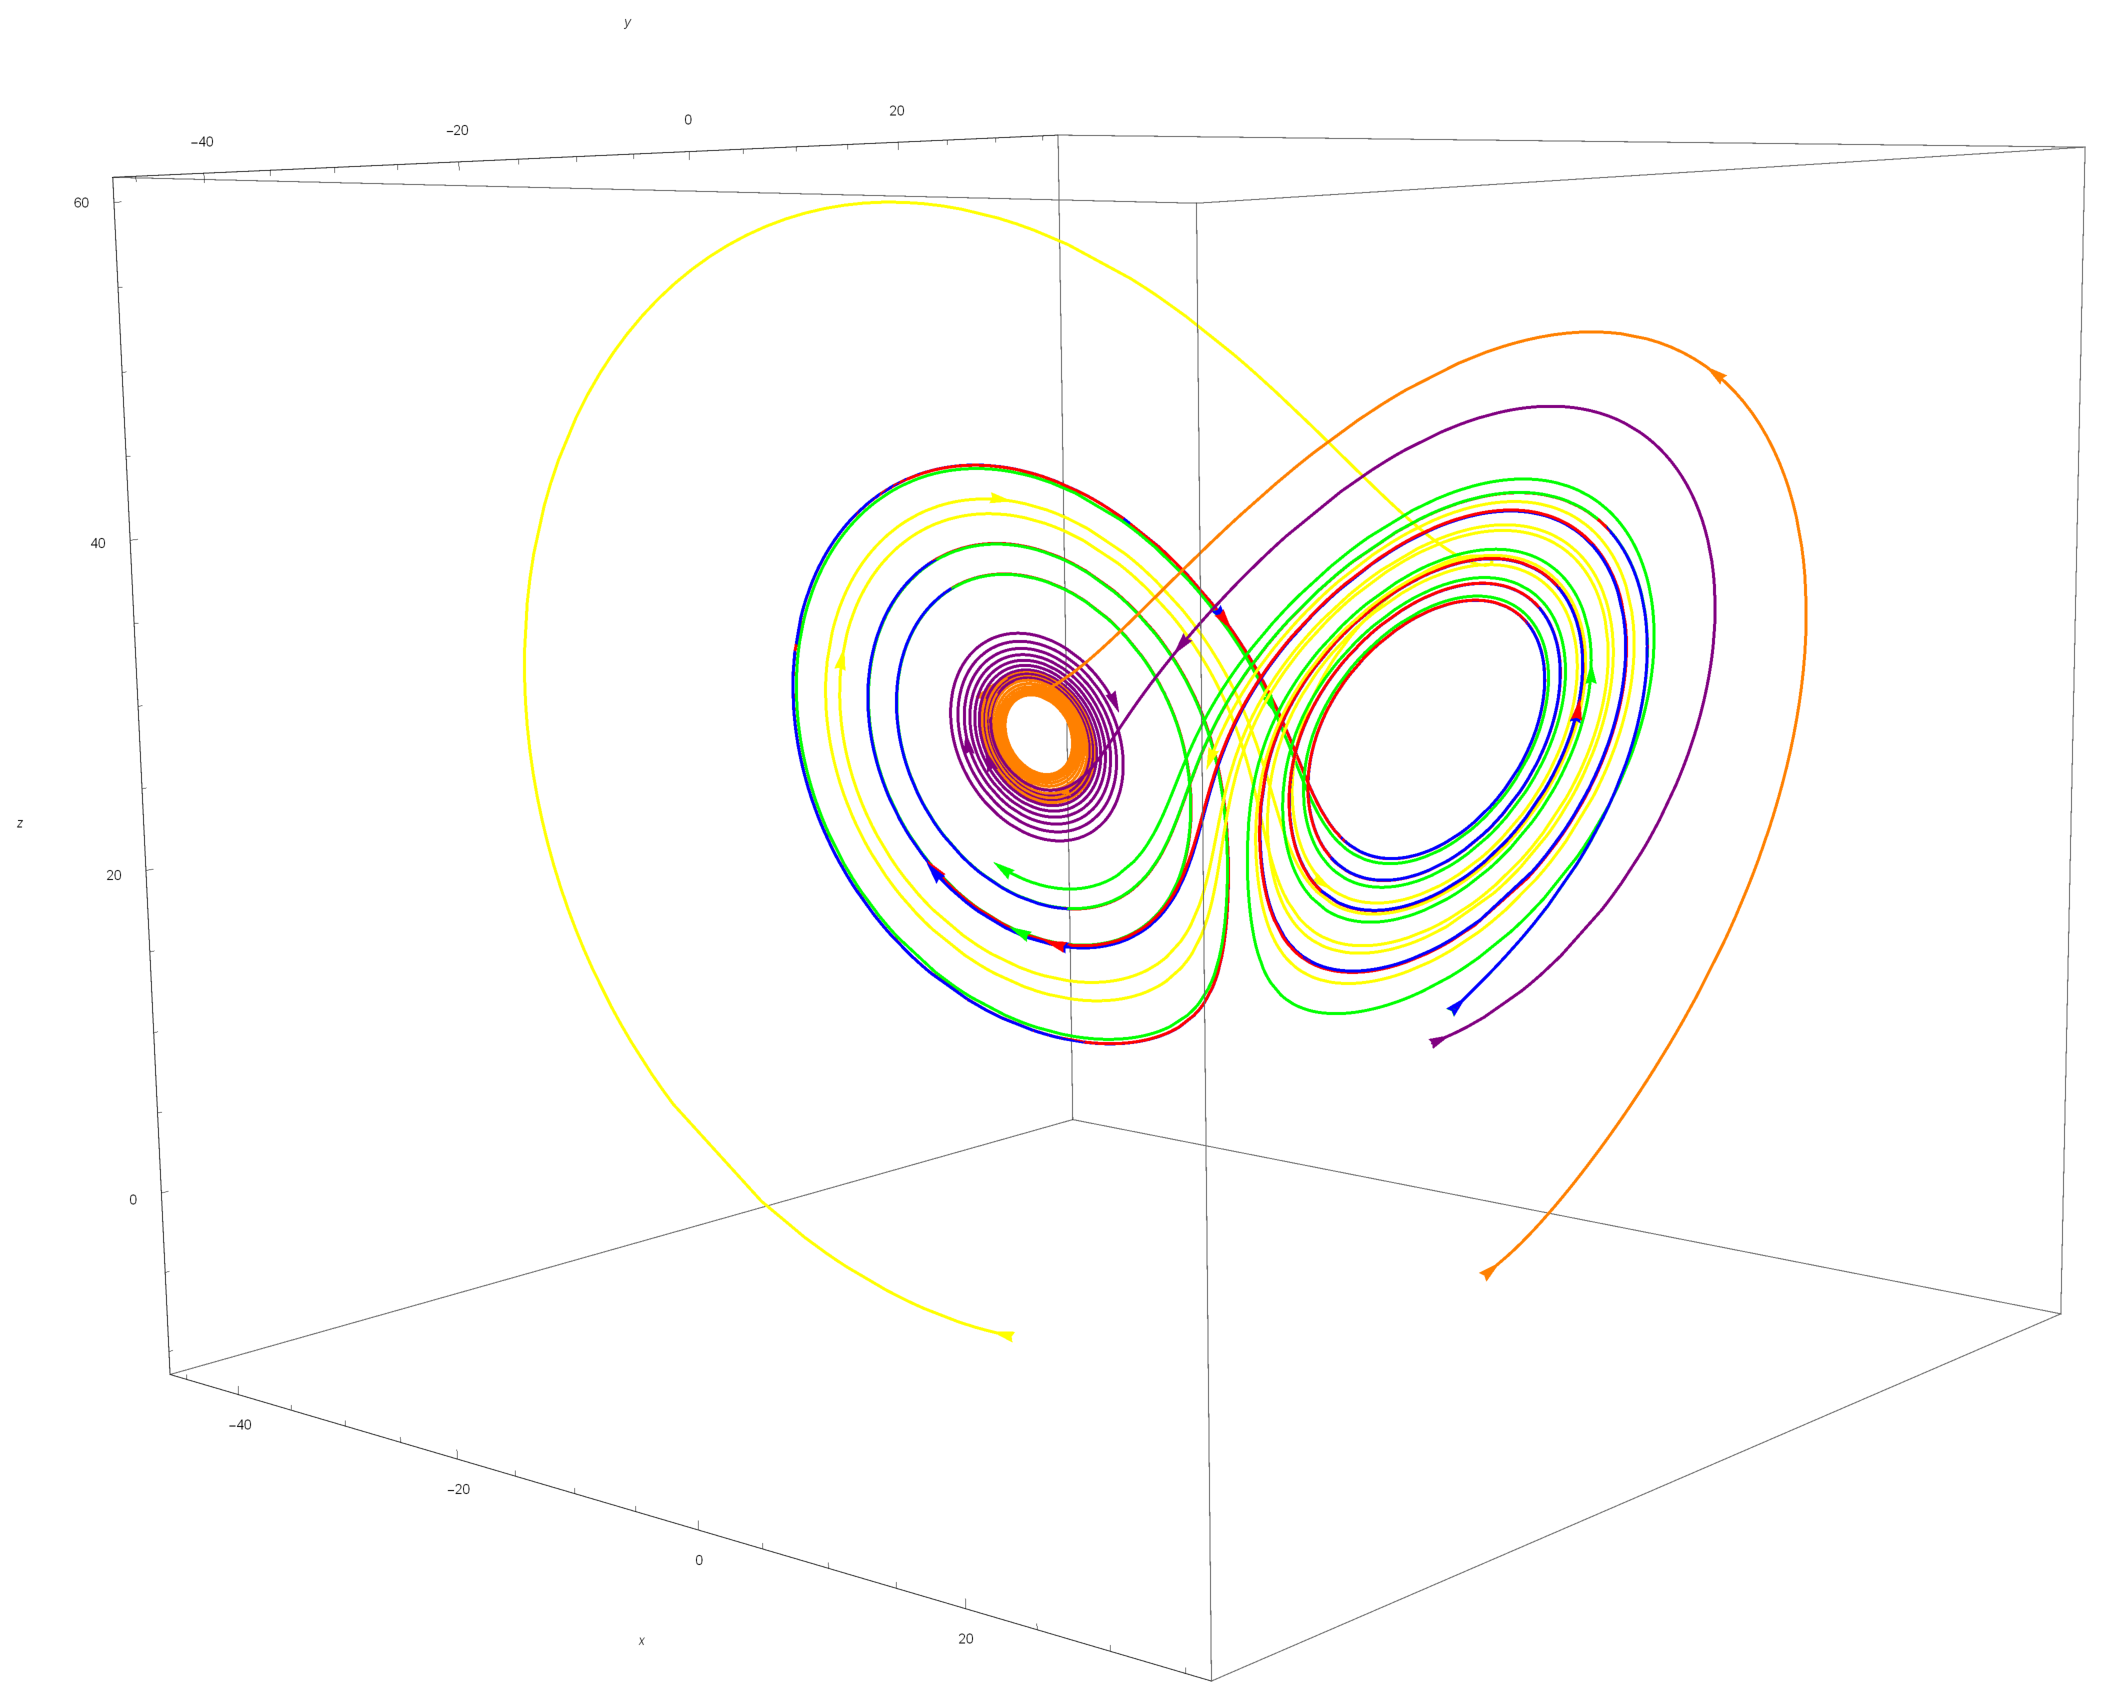
\includegraphics[width=0.75\textwidth]{r28.eps}
  \caption{Trajectories for r = 28}
  \label{fig:r_28}
\end{figure}

\begin{figure}[h]
  \centering
  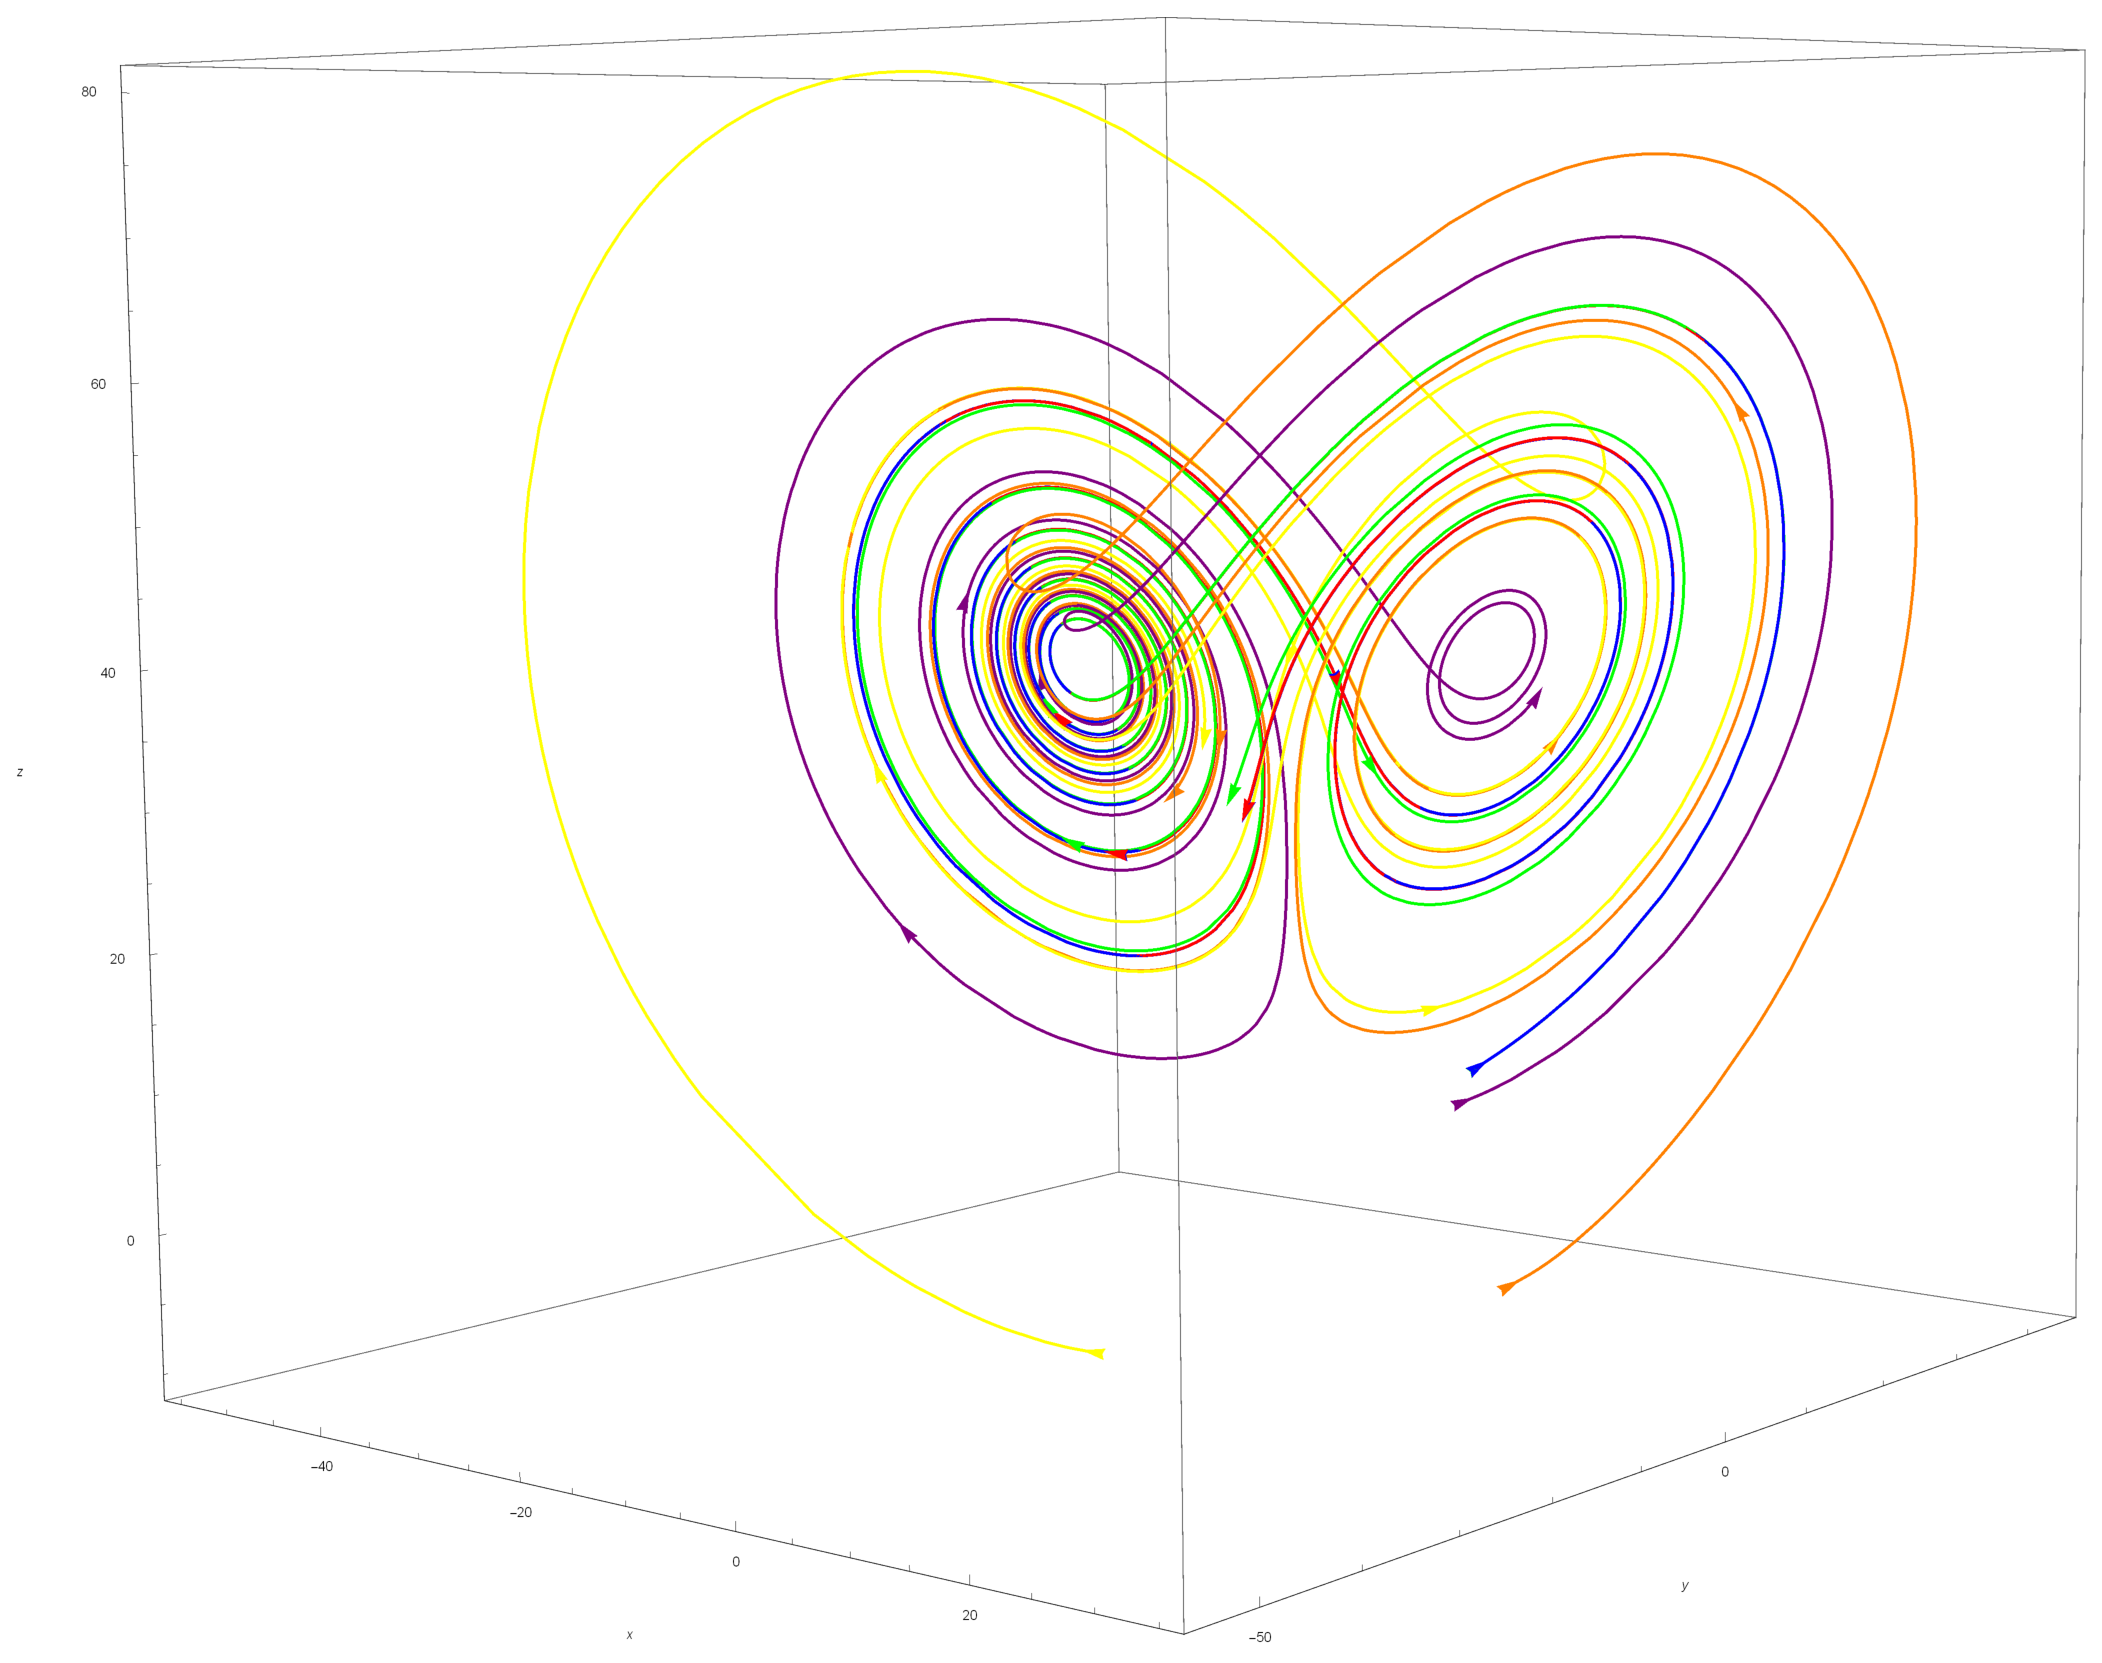
\includegraphics[width=0.75\textwidth]{r40.eps}
  \caption{Trajectories for r = 40}
  \label{fig:r_40}
\end{figure}

Once \(r > r_H \approx 24.7 \), chaotic behavior begins to appear.
\begin{thebibliography}{9}

\bibitem{strogatz15}
  Steven H. Strogatz,
  \emph{Nonlinear Dynamics and Chaos: with Applications to Physics, Biology,
Chemistry, and Engineering},
  Westfield Press, Colorado,
  2nd edition,
  2015.

\bibitem{sparrow82}
  Colin Sparrow,
  \emph{The Lorenz Equations: Bifurcations, Chaos, and Strange Attractors}
  Springer-Verlag, New York,
  1982.
\end{thebibliography}
\end{document}
